\documentclass{sigchi}

% Arabic page numbers for submission. 
% Remove this line to eliminate page numbers for the camera ready copy
%\pagenumbering{arabic}

% Load basic packages
\usepackage{balance}  % to better equalize the last page
\usepackage{graphics} % for EPS, load graphicx instead
\usepackage{times}    % comment if you want LaTeX's default font
\usepackage{url}      % llt: nicely formatted URLs
\usepackage{todonotes}

% Load basic packages
%\usepackage[pdftex]{graphicx}
%\usepackage{amsmath, amssymb}
\usepackage{verbatim}
%\usepackage{tabularx}
\usepackage{mdwlist} %compact lists
%\usepackage{algorithm}
%\usepackage{algpseudocode} % program code

\usepackage{listings}

% llt: Define a global style for URLs, rather that the default one
\makeatletter
\def\url@leostyle{%
  \@ifundefined{selectfont}{\def\UrlFont{\sf}}{\def\UrlFont{\small\bf\ttfamily}}}
\makeatother
\urlstyle{leo}


% To make various LaTeX processors do the right thing with page size.
\def\pprw{8.5in}
\def\pprh{11in}
\special{papersize=\pprw,\pprh}
\setlength{\paperwidth}{\pprw}
\setlength{\paperheight}{\pprh}
\setlength{\pdfpagewidth}{\pprw}
\setlength{\pdfpageheight}{\pprh}

% create a shortcut to typeset table headings
\newcommand\tabhead[1]{\small\textbf{#1}}

% to give it a fighting chance of not being over-written, 
% since its job is to redefine many LaTeX commands.
\usepackage{ifpdf}
\ifpdf
\usepackage[pdftex]{hyperref}
\else
\usepackage{hyperref}
\fi
\hypersetup{
pdftitle={SIGCHI Conference Proceedings Format},
pdfauthor={LaTeX},
pdfkeywords={SIGCHI, proceedings, archival format},
bookmarksnumbered,
pdfstartview={FitH},
colorlinks,
citecolor=black,
filecolor=black,
linkcolor=black,
urlcolor=black,
breaklinks=true,
}

\graphicspath{{pictures/}}

% Use this command to override the default ACM copyright statement (e.g. for preprints). 
% Consult the conference website for the camera-ready copyright statement.
 \toappear{\scriptsize Permission to make digital or hard copies of all or part of this work for personal or classroom use is granted without fee provided that copies are not made or distributed for profit or commercial advantage and that copies bear this notice and the full citation on the first page. Copyrights for components of this work owned by others than the author(s) must be honored. Abstracting with credit is permitted. To copy otherwise, or republish, to post on servers or to redistribute to lists, requires prior specific permission and/or a fee. Request permissions from Permissions@acm.org. \\
 {\emph{UIST'13}}, October 8--11, 2013, St. Andrews, United Kingdom. \\
 Copyright \copyright~2013 ACM 978-1-4503-2268-3/13/10...\$15.00. \\
http://dx.doi.org/10.1145/2501988.2502007}
 
\clubpenalty=10000 
\widowpenalty = 10000 


\newcommand{\eg}{e.g.,\ }
\newcommand{\ie}{i.e.,\ }
\newcommand{\lablet}{Lablet\ }
\newcommand{\lablets}{Lablet's\ }
\newcommand{\labactivity}{Lab Activity\ }
\newcommand{\labactivities}{Lab Activities\ }
\newcommand{\wysiwyg}{\mbox{WYSIWYG}\ }
\newcommand{\dragndrop}{drag and drop\ }


% End of preamble. Here it comes the document.
\begin{document}

\title{Lablet: A Mobile Learning Enviornment}

\numberofauthors{1}

\author{
	\alignauthor \mbox{Clemens Zeidler, Anna Yang, Kasper van Wijk}\\
		\affaddr{University of Auckland}\\
		\affaddr{38 Princes Street}\\
		\affaddr{Auckland 1010, New Zealand}\\
		\email{\{clemens.zeidler, a.yang, k.vanwijk\}@auckland.ac.nz}
}

\maketitle

%\tableofcontents

\begin{abstract}
%TODO Anna
\end{abstract}

\category{H.5.2}{User Interfaces}{Graphical user interfaces (GUI)}


\keywords{e-learning; mobile devices; physics experiments; electronic handouts}


\section{Introduction}
%Kasper: What do our (or any physics department's) labs aim to accomplish now (on paper), what does the lablet provide/add? Sensing, and analysis capabilities would be the two main things.
%A connection with "modern wired life" (there may be  a better term) is maybe another important consideration.

The increasing ownership and availability of mobile devices with
advanced sensors equip anyone interested in physics to get creative
with scientific inquiries.  While mobile technologies offer
opportunities to transform teaching and learning
practices~\cite{karnad2014trends, Kukulska2010}, relatively few mobile
projects have been designed that could facilitate social learning and
user-generated content~\cite{Frohberg2009}. 

Discuss \cite{Kearney2012,Etkina2006,Millar2002,Trumper2003}

The Auckland Lablet provides an active learning environment for
Physics experimentation on an Android tablet.  The intuitive interface
and the rich sensor suite of touch screen tablets create a powerful
learning tool built on commodity hardware.  Lablet users capture and
analyse data in and outside our teaching laboratories; Lablet modules
leverage a range of internal sensors in the tablet, and the fully
customisable Lablet environment can guide students through physics
experiments.

Lablet users optimise their time with learning hands-on Physics.  In
addition, Lablet creates a “paperless workflow” for grading and
student feedback, so that the Lablet maximises the time that lab
instructors spend interacting with students.

The goal of this project is to facilitate the growth of a community of
Lablet users in high schools, studio-based learning
environments, and flipped classrooms.  Lablet’s low cost and
versatility create a wealth of opportunities for playful independent
exploration.  
%Imagine students combining Doppler analysis and video
%motion tracking data of cars on a busy road, using an accelerometer in
%an elevator to measure the height of a building, or analysing the
%motion of a ball on a sport field.

The Auckland Lablet is open source; our applications and source code
are freely available for use and modification.  The current release
includes video, audio and accelerometer capturing and analysis
modules.  Future releases will exploit the ambient light sensors,
compasses, gyroscopes and GPS receivers found in tablets, as well as
purpose-built Arduino-based Bluetooth connected sensors.

Next we introduce the internal tablet sensors supported in Lablet as a
new Mobile learning environment, and the analysis capabilities that
accompany the sensing. We then discuss possible experiments, with data
acquired by supported sensors and analysed on the tablet. Finally, we
present the scripting language of Lablet to link experiments with
individual sensors or embed one or more experiments in what we call
``activities'' in Lablet.

In a classical laboratory class students usually get a paper-based handout that guides them through the class.
The handout can include instructions, questions and other tasks.
For example, the handout can instruct students to manually calculate the velocity of a moving object using \lablets motion analysis module.
The desired learning outcome for this experiment could be to understand how to calculate the velocity from consecutive position measurements and discuss the velocity time graph.
To do so data can be exported from the mobile device and analyzed on a computer.
However, this complicates the laboratory class since more equipment is required and students needs to learn to use the analysis software.
Another way to analysis the data is to calculate the velocity manually using pen, paper and a
calculator.
The drawback of this method is that students have to repeat a relative simple task multiple time and the results and because teachers have to recalculate the results they are difficult to verify.
Either way, students have to spend time with tasks that are not part of the desired learning outcome.

\subsection{Contributions}
Our contributions can be summarised as follows:

\begin{enumerate}
\item \lablet, a novel physics learning environment for mobile devices.
\item Lab Activities.
\end{enumerate}

\section{Related Work}
% Web camera as a measuring tool in the undergraduate physics laboratory and Investigating viscous damping using a webcam 
For example, a web camera has been used to analyze diffusion of ink drop in water, damped oscillations of a pendulum, diffraction patterns~\cite{Nedev2006} and mass oscillating in a viscous fluid~\cite{Shamim2010}.
% Cellular Phones Helping To Get a Clearer Picture of Kinematics 
The kinematic of a water jet from a hose can be studied by taking a photo of the scene using a mobile device~\cite{Falcao2009}. \lablet users have the option to record video at different resolutions and
frame rates.

Lablet's motion analysis module is inspired by tracker\todo[inline]{cite from the webpage Conference Presentations...}\footnote{\url{http://physlets.org/tracker/}}.
However, tracker does only supports one sensor and an external camera is needed to record a video.
% sound:

% acoustics
Using a fast Fourier transformation the different types of sounds such as a tone, a periodic and none-sinusoidal vibration pattern, noise and impulse can be analyzed using the microphone of a mobile device~\cite{KuhnAcousticPhenomena2013}.

% accustic measurement of a bouncing ball
Mobile devices can also be used to record the sound of an bouncing ball~\cite{Schwarz2013Acoustic}.
From the time difference of the bounces and the initial height the gravitation can be determined.

% bell-jar
The sound propagation in vacum can be demonstrated by hanging a ringing mobile phone into bell-jar~\cite{CaleonBellJar2013}.


% accelerometer:

% Analyzing free fall with a smartphone acceleration sensor
Another experiment proposes to facilitate the accelerometer of a mobile device to analyze a free fall by dropping the mobile device on a cushion~\cite{VogtFreeFall2012}.
% Analyzing spring pendulum phenomena and radial acceleration with a smartphone acceleration sensor
Similar, a mobile device can be used to record acceleration of a spring pendulum, a coupled spring pendulum~\cite{KuhnPendulum2012}, a free and a damped harmonic oscillation~\cite{Castro2013}.
By rotating the mobile device the radial acceleration can be measured~\cite{VogtRadialAcc2013}.


% other sensors:

% The optical mouse for harmonic oscillator experimentation
An optical mouse can be used as an extremely cost-effective displacement sensor, for example, to measure the damped harmonic oscillations~\cite{Ng2005}.

% oscilloscope
Mobile devices can be act a portable oscilloscopes~\cite{Forinash2012}.
The microphone jack can be used as an input.
The recorded data can be Fourier analyzed.

% Smartphones—Experiments with an External Thermistor Circuit
The microphone jack can also be used as an input for external sensors such as a thermistor~\cite{Forinash2012}.

% Wiimote
The Wiimote sensor can been used to track multiple objects simultaneously, \eg to observe a spring system with multiple coupled masses~\cite{Skeffington2012}.

% A simple demonstration for exploring the radio waves generated by a mobile phone
A mobile phone can also be used as a radio wave source that can be measured using a simple wave detector~\cite{Hare2010}.


\section{Sensors}\label{sec:Sensors}
\lablet uses the build in sensors of mobile devices to record data.
Data from multiple sensors can be recorded in parallel, for example, to record the an visual and acoustic data of an event.
Currently, these sensors are the camera, the microphone and the accelerometer.
The quality and abilities of a sensor depends on the manufacture and the used model.
For this reason we only discuss the general properties of these sensors and discuss possible limitations based on our experiences using \lablet in the lab classes.

\paragraph{Camera}
Modern mobile devices are usually equipped with at least one camera that can record videos at a reasonable high resolution.
In general cameras in mobile devices do not record at a fix recording frame rate but only try to reach a target frame rat.
From our experiences many cameras are able to record with a reasonable stable frame rate between 25 and 30 fps.
However, a recording frame rate of 30fps is not uncommon.
In other words experiments can be recorded with a time resolution of 34-40ms.
\todo[inline]{is that called time resolution?}
% I don't know what exactly going on so I'm a bit vage here and do not name a certain component for the problem:
Failing to record a video frame usually results in duplicated frames in the video file, \ie the missing frame is compensated by another frame.

% blur of fast moving objects
A common problem with cameras in mobile devices is that fast moving object become blurry in the video.
This can effect how precise the position of a moving object in a video can be detected.
Usually a good illumination of the recorded scene can help to reduce the blur effect.

% long videos
Recording long videos can result in very large video files that might exceed the storage of the mobile device.
For example, recording a video at 1280x800@30fps results in a mp4 file roughly of the size of 4.2 Gb per hour.
In order to reduce the disk requirements \lablet allows to lower the recording frame rate or video resolution.
\lablet allows to record video with a video frame rate down to 0.1 fps but theoretically there is now lower limit for the recording frame rate.
This allows to record long video with either a high video- and a low time-resolution or with a low video- and a high time-resolution.

\paragraph{Microphone}
Common microphones in mobile devices are able to record audio data with a sampling rate of 44100Hz.
This allows the un-aliased recording of sound from roughly 20Hz to 22000Hz which is corresponds to the hearing range of humans.
Note, since microphones in mobile devices are designed to record the human audible spectrum a microphone might be less sensitive for certain frequency ranges.
For example, high frequencies are less important for hearing than low frequencies.

\paragraph{Accelerometer}
Accelerometer in mobile devices usually detect accelerations in x, y and z direction.
Since there are many different accelerometers used in mobile devices we just give some example specifications to illustrate the capabilities of such accelerometers.
With the Galaxy Tab4 we were able to record $\sim100$ accelerometer data points per second.
The BMA180\footnote{\url{http://www.sensorsmag.com/product/mems-accelerometer-bosch-sensortec}}, a microelectromechanical system (MEMS) accelerometer can detect accelerations of $0.00025g$ and a tilt change in the field of gravity of $0.25^{\circ}$

%Lablet calculate a resulting total acceleration value from these three
%\[
%a_{total} = \sqrt{a_x^2 + a_y^2 + a_z^2}
%\]

\section{Analysis Modules}\label{sec:AnalysisModules}
Recorded sensor data can directly be analysed using Lablet's analysis modules.
Moreover, external video or audio data can be imported to \lablet and then be analysed within \lablet.
Currently, there are three analysis modules available that are presented in the following.

\subsection{Motion Analysis Module}
The motion analysis module can be used to analyse a moving object in a recorded video.
The main idea here is to step throw the video frame by frame and mark the position of the moving object.
Using the so gathered object position data in combination with the time data from the video frames the the velocity and acceleration of the moving object can be derived.

%\subsubsection{Motion Tracking}
\lablet supports to automatically track an object in a recorded video.
After marking an object in a video frame \lablet is able to mark this object automatically in the subsequent frames.
Object tracking works best for object with high contrast to their background.

% video settings
\lablet allows to configure what part of the video should be analysed, \ie the video can be cropped to an interesting region.
Furthermore, the user can choose at what frame rate the video should be analysed.
For example, if only every second frame needs to be analysed the analysis frame rate can be halved (see Figure~\ref{fig:MotionAnalysisSettingsScreen}).

\begin{figure}
  \centering
  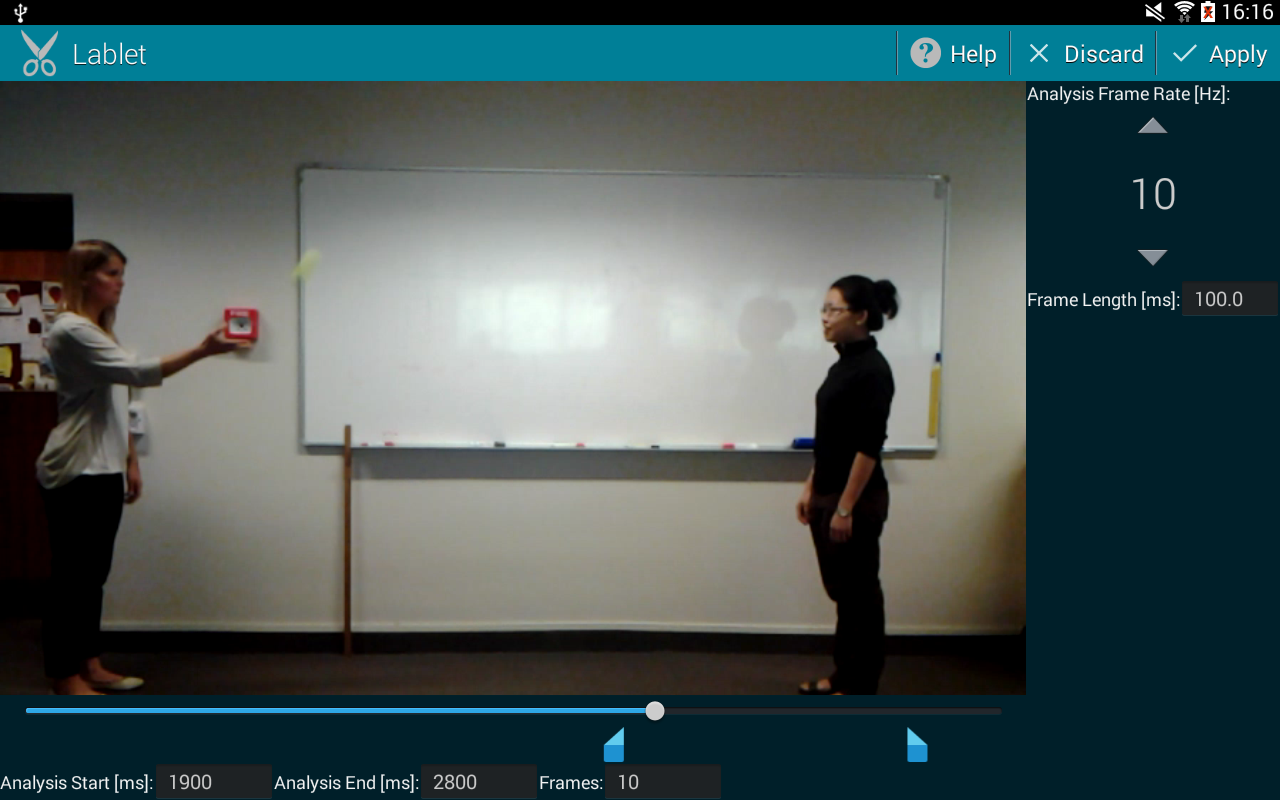
\includegraphics[width=.99\columnwidth]{MotionAnalysisSettings}
  \caption{Motion analysis settings screen.
  On the left bottom the part of the video that contains the experiment can be selected.
On the right side the analysis frame rate can be adjusted.\label{fig:MotionAnalysisSettingsScreen}}
\end{figure}

% length scale
One problem that arise when analysing a moving object in a video is that in general the distance of the object to the camera is unknown and thus the travelled distance of the object can not be determined.
To solve this problem, \lablet assumes a reference object with known size that is placed in the recorded scene.
By marking the reference object using a linear scale and by specifying the length of the scale \lablet can derive the spacial extend of the recorded scene (see Figure~\ref{fig:MotionAnalysis}).
% how to get optimal results
Note, that for optimal results the video should be recorded parallel to the plane of the moving object and the reference object should be located in that plane.

% origin
Optionally, the coordinate system of the recorded scene can be defined, \ie the position and the orientation of the coordinate system can be specified (Figure~\ref{fig:MotionAnalysis}).
Furthermore, the $x$ and $y$ axes can be swapped.
This can, for example, be helpful to analyse object that are moving from right to left.

\begin{figure}
  \centering
  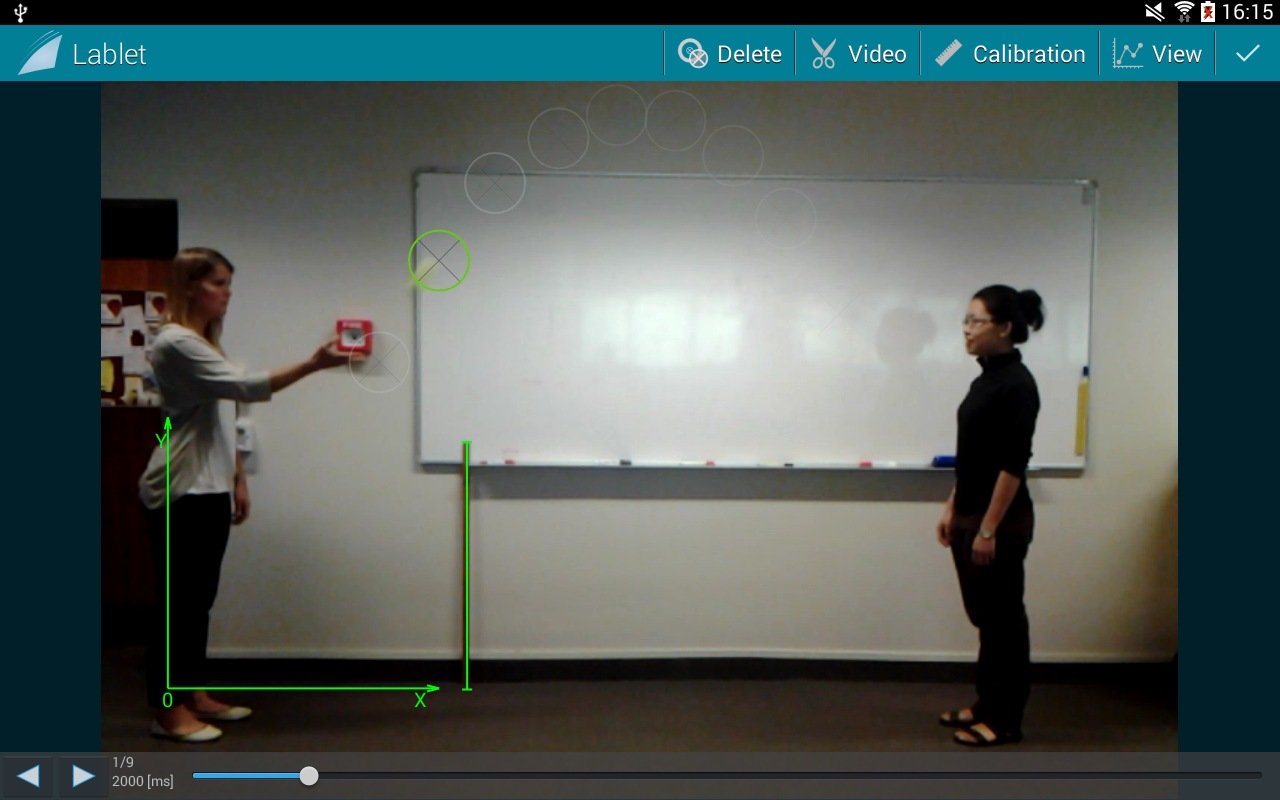
\includegraphics[width=.99\columnwidth]{MotionAnalysis}
  \caption{Motion analysis screen.
  The green length scale can be used to calibrate the size of the video scene.
  The coordinate system can be used to set origin and orientation of the video scene.\label{fig:MotionAnalysis}}
\end{figure}

\subsection{Frequency Analysis Module}
The frequency analysis module performs a discrete Fourier analysis on recorded audio data.
This can be used to discuss the frequency spectrum of a sound source.
For example, to analyse the Doppler effect of a moving sound source.
The data from the Fourier analysis is visualized in a frequency map that displays the frequency data versus the recording time (see Figure~\ref{fig:FrequencyAnalysis})
The frequency analysis module allows to change various parameter of the discrete Fourier analysis which makes it a good tool to demonstrate a discrete Fourier analysis to students.

% cursors
In order to highlight interesting points in the frequency map the frequency analysis module allows to position an arbitrary number horizontal and vertical cursors.
This can, for example, be used to measure the period of an audio signal or the frequency difference of
a Doppler shift experiment.

% visualization
To visualize very small frequency changes the user can changing the colour contrast and brightness.
Furthermore, the frequency map is zoom-able and makes it possible to magnify interesting data points.

% details
To perform a discrete Fourier analysis on the recorded audio data the audio data is first partitioned into fix sized data windows.
For each window first a Hamming window function and then a discrete Fourier analysis is performed.
The discrete Fourier analysis is then performed on each of these windows.
The window size as well as the overlap of two consecutive windows can be configure.
For example, a window overlap of 0\% means that two consecutive windows are directly adjacent while an overlap of 50\% means that the second half of the previous window is the first half of the following window.

\begin{figure}
  \centering
  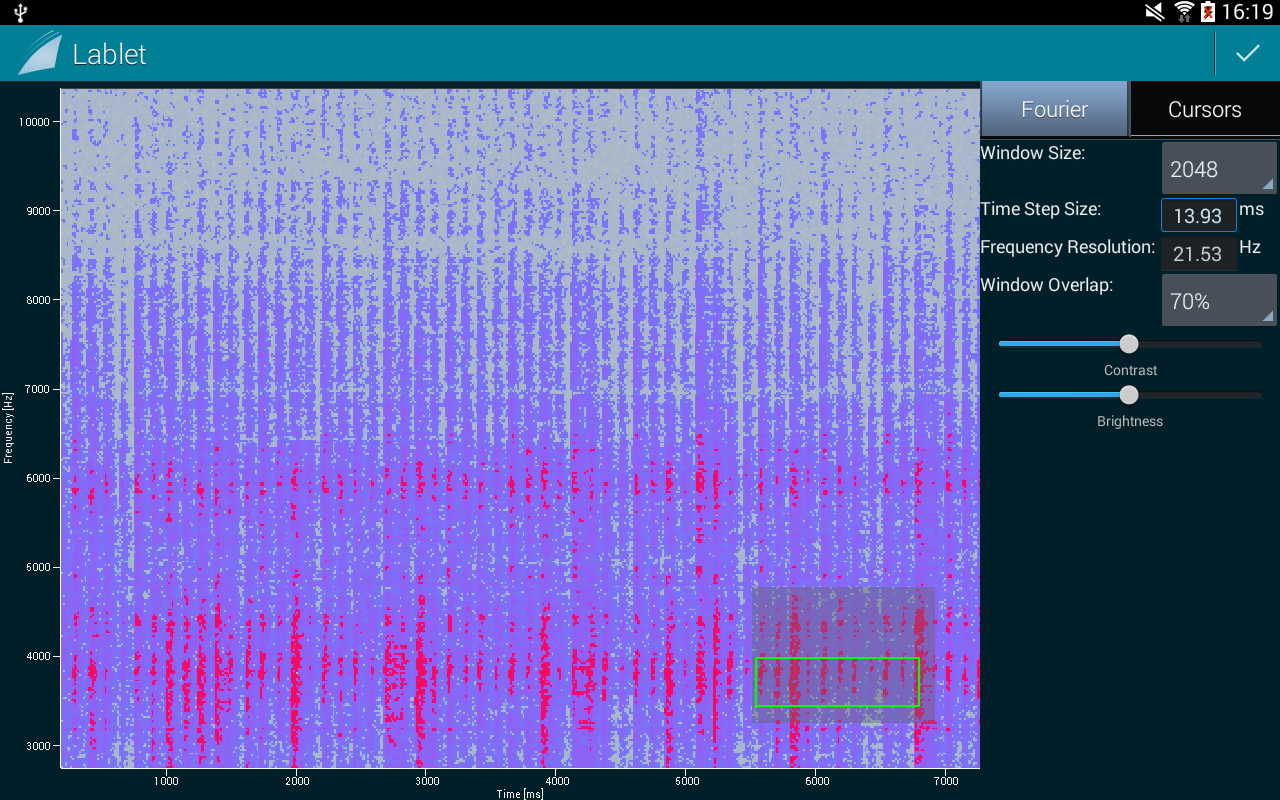
\includegraphics[width=.99\columnwidth]{FrequencyAnalysis}
  \caption{Frequency analysis screen.
  The results of a discrete Fourier analysis is displayed versus the recording time.\label{fig:FrequencyAnalysis}}
\end{figure}

% what window size and window overlap do
In the following we discuss how the window size and the window overlap affects the time and the frequency resolution of the frequency map. 
For a given sampling rate $f_s$ and a window size of $n$ samples, the time between two windows is
\[
\Delta t_w = n / f_s
\]
This means the time resolution of the time frequency plot is high if the window size is small.
When using a percental window overlap $p$ this time deceases further to
\[
\Delta t_w = n / f_s * (1 - p / 100)
\]
Since the hamming window function is sensitive to the window overlap, in practice, some frequency changes become more visible when using a certain window overlap.

% frequency resolution
% TODO: is frequency resolution the right term?
The frequency resolution is given by
\[
\Delta f = f_s / (n - 1)
\]
Thus, the trade-off of increasing the time resolution by decreasing the window size is that the frequency resolution degrades.
In practice a good compromise has to be found that gives good results for a certain problem.

\subsection{Accelerometer Analysis Module}
While the motion analysis module is able to determine velocity and acceleration of a moving object, the accelerometer analysis module can be used to calculate velocity and displacement of the mobile device from the measured acceleration.
To calculate the mobile device's velocity the acceleration has to be integrated over the time and to calculate the displacement another integration has to be performed.

% problem
The main problem when integrating acceleration data is that small measuring errors or uncertainties of the initial acceleration are propagate in every integration step and a drift in the integrated data can be observed.
The problem gets even worse when the so calculated velocity is integrated a second time.
For example, even if the mobile device is at rest at the begin of the measurements one can not assume that sensor is probably calibrated to report the gravity of the earth.
This initial offset contributes linear to the velocity and quadratic to the displacement calculation.

% calibration
The integration problem described above makes it very hard to perform meaningful velocity or displacement measurements.
However, the accelerometer analysis module allows to adjust the initial acceleration and allows students to experience the effect on the resulting velocity and displacement.
Furthermore, trying reasonable initial acceleration values students can get qualitative results that can then be compared to the expected results.

% using external knowledge
Another way to tackle the integration problem is to use additional knowledge about the measured movement.
For example, Figure~\ref{fig:AccelerometerAnalysis} shows the measurement of a mobile device travelling in an elevator from the top level to the ground floor.
Known is that at the start and the end of the journey the elevator and thus the mobile device is at rest.
Choosing the initial acceleration in a way that these conditions are met in the velocity data, one can actually observe that the elevator moved with a constant velocity between a acceleration and deceleration phase.
Furthermore, the measured displacement is compatible with the height of the building.

\begin{figure}
  \centering
  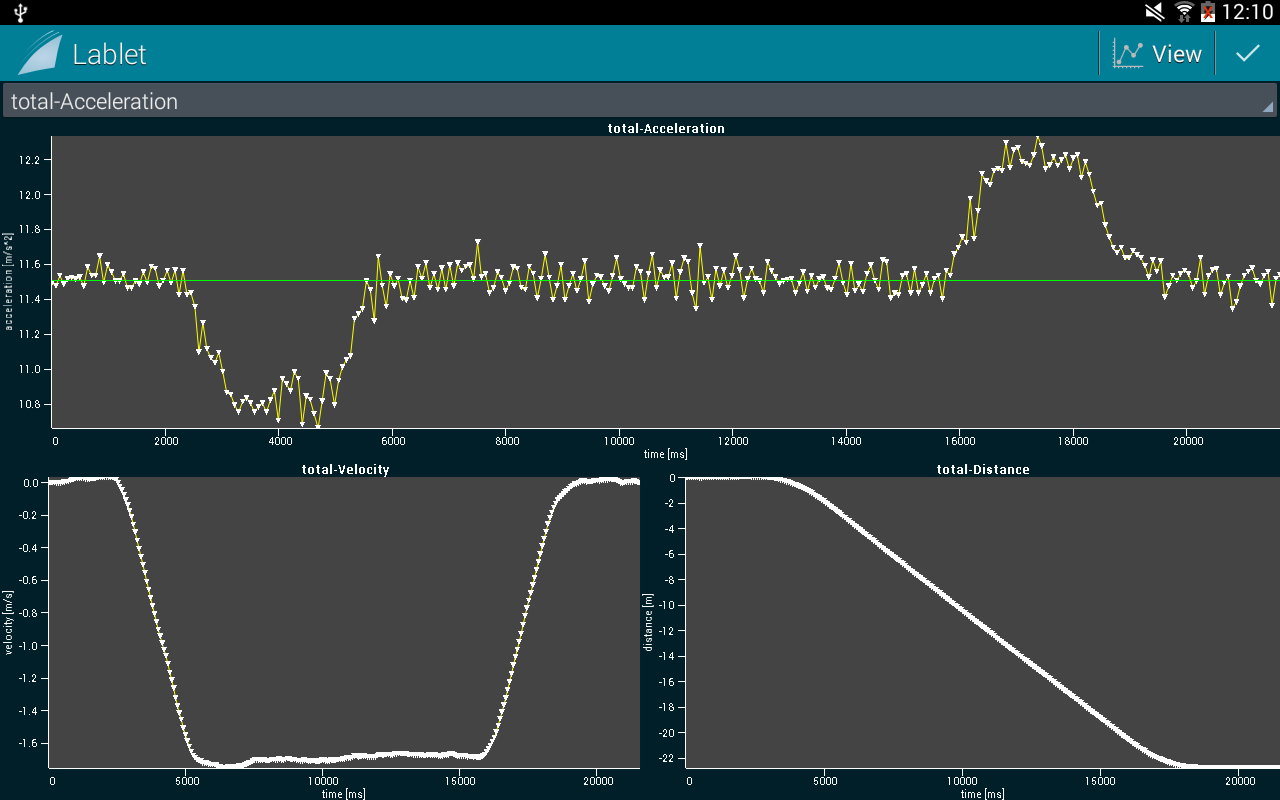
\includegraphics[width=.99\columnwidth]{AccelerometerAnalysis}
  \caption{Accelerometer analysis screen.  In the top time
    acceleration the experimenter can calibrate the initial
    acceleration at rest.  From this the velocity and distance graphs
    are calculate (bottom left and bottom
    right).\label{fig:AccelerometerAnalysis} }
\end{figure}


\subsection{Data Export}
The here presented analysis modules that are currently supported by \lablet are designed for a certain type of analyses.
To perform other analyses external tools has to be used.
For that reason \lablet allows to export measured sensor data as well as the results of \lablets analysis modules.

\section{Lab Activities}
\todo[inline]{move this first bit into the introduction?}
In laboratory classes students often need instructions that guide them through the experiments.
\lablet introduces {\em \labactivities} to provide students with information and instructions directly on the tablet.
A \labactivity can include a multitude of elements such as instructions, questions, experiments or graphs.
Furthermore, \lablets sensor experiments and analysis modules can be embedded into a \labactivity. 
\labactivities are comparable to classical paper-based handouts.
\labactivities can be created by teachers and are highly customizable.

\begin{figure}
  \centering
  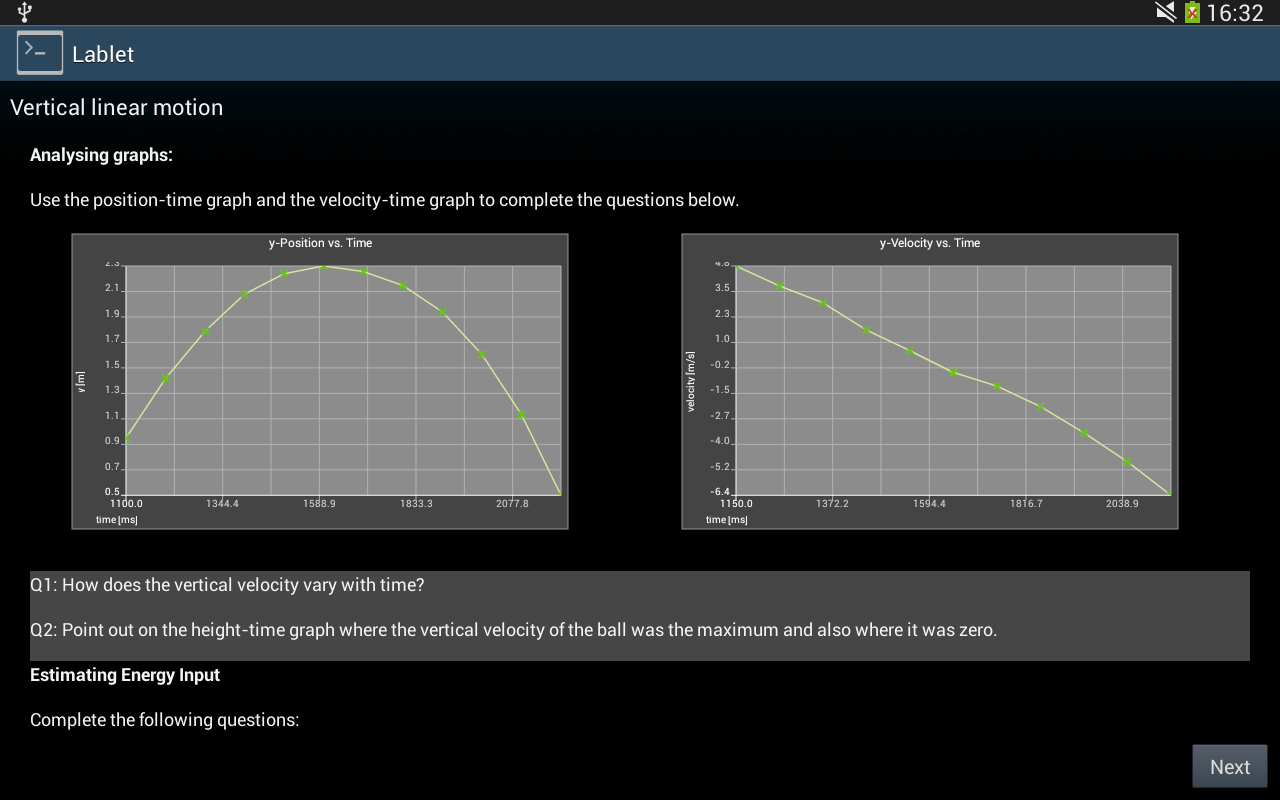
\includegraphics[width=.99\columnwidth]{LabActivitySheet}
  \caption{\label{fig:LabActivitySheet}Sheet from a Lab Activity containing various different elements.} 
\end{figure}

% desciption of the Lab Activities UI
Each \labactivity can have multiple sheets.
Each sheet can have an unlimited number of elements.
Some elements requires to be completed before students can proceed to the next sheet.
For example, check boxes needed to be ticked before the next sheet becomes available.
Users can easily navigate between sheets using a simple horizontal swipe gesture.
Figure~\ref{fig:LabActivitySheet} shows an example of a sheet containing various different elements.

% layout
Lablet comes with a powerful but simple layout model to position elements on a sheet.
Elements can be placed in horizontal or vertical boxes that can be further nested to create more complex layouts.
For example, the main layout in Figure~\ref{fig:LabActivitySheet} is a vertical box while the two graphs are placed in a horizontal box.

\subsection{Elements}
In the following a brief overview of the the available \labactivity elements that can be placed on a sheet is given.

\paragraph{Header}
The header element can be used to mark a new section on the sheet.

\paragraph{Text}
The text element displays some text and can be used for instructions or other information.

\paragraph{Check Box}
The check box element has some descriptive text and a check box.
All check boxes on a sheets need to be checked before the next sheet is activated.

\paragraph{Question}
The question element is a simple line of text that can be used to ask a question.

\paragraph{Question with Answer Text}
Additionally to the basic question element this element contains a field for text input.

\paragraph{Sensor Experiment}
The sensor experiment element starts a camera, a microphone or an accelerometer sensor experiment (see Section~\ref{sec:Sensors}).

\paragraph{Data Analysis}
The experiment analysis element starts one of \lablets analysis modules (see Section~\ref{sec:AnalysisModules}) to analyse recorded data.

\paragraph{Graph}
The graph element displays data from the motion analysis module in a 2D graph.
The graph axes can be configured to show time, position, velocity or acceleration data.

\paragraph{Derivation}
The derivation element let students calculate velocity and acceleration from motion data gathered in the motion analysis module.
%This element uses three successive data points to calculate the acceleration value from the two velocity points.
Students have calculate the correct numeric values and select the correct unit for velocity and acceleration.
\lablet automatic verifies the results.
Once a few sample points are calculated correctly the remaining values are calculated automatically.

\paragraph{Potential Energy}
This potential energy element let the students estimate the potential energy of a mass at a certain height.
The student then exercise the unit transformation from Joule to Calories.
\lablet automatically verifies the results.

\subsection{Editing Lab Activities}
Teachers can specify \labactivities in a plain text file.
This text file can be imported and managed into \lablet.
The following listing shows a small example of a \labactivity specification containing a single sheet and a few elements.

\begin{lstlisting}
Lablet = {
    interface = 1.0,
    title = "Lab Activity Demo Sheet"
}
 
function Lablet.buildActivity(builder) {
    -- comment: add a single sheet
    sheet = builder:create("Sheet")
    builder:add(sheet)
    sheet:setTitle("Physics Laboratory")
    sheet:addHeader("Lab equipment:")
    sheet:addText("Do you have:")
    sheet:addCheckQuestion("metre rule")
    sheet:addCheckQuestion("ball")
}
\end{lstlisting}

\section{Conclusion}
In this paper we presented \lablet, a new physics learning environment for mobile devices.
\lablet allows to record data using common sensors of modern mobile devices, \ie camera, microphone and accelerometer.
Using three build in analysis modules, \ie motion analysis, frequency analysis and accelerometer analysis, recorded data can analysed directly on the mobile device.
\lablets \labactivities enables teachers to define complex electronic handouts that guide students through laboratory classes.
\labactivities supports exercise tasks that give direct feedback to the students.

\lablet makes it easy to perform and analyse experiments outside of the classical laboratory.
\labactivities reduces repetitive tasks such as drawing plots and calculating data so that students have more time to discuss results with each other and the teacher.

\paragraph{Future Work}
In future work we plan to support more internal and external sensors such as gyroscope, thermometer or adrino sensors.
While \lablet already supports three analysis modules one can think of more modules for different type of analyses or combined analyses.
For example, \lablet supports to record video and audio data at the same time but can only analyse the data separately.
Combining both analyses would make it possible to map sound events to visual events.
For the \labactivity we plan to support more elements and task.
Furthermore, we like to make it easier for teachers to create new \labactivities.


\bibliographystyle{acm-sigchi}
\bibliography{BibEntries}

\end{document}


\begin{comment}
\section{Experiments}
In this section we summarize a possible set of experiments that can be
conducted using Lablet.

\section{Improved Learning Environment}
% TODO Anna:
- face to face 
- avoiding repeatative tasks

\section{Evaluation}

\subsection{Observations}
Students use calculators and pen and paper to fill speed and
accelerator values.  That is good because they real have to get into
the problem; Lablet does not do the core part for you it is just a
tool that helps learning.
\end{comment}

